%% Copernicus Publications Manuscript Preparation Template for LaTeX Submissions
%% ---------------------------------

\documentclass[esurf, manuscript]{copernicus}



%% Journal abbreviations (please use the same for discussion papers and final revised papers)

% Earth Surface Dynamics (esurf)
% Geoscientific Model Development (gmd)

%% \usepackage commands included in the copernicus.cls:
%\usepackage[german, english]{babel}
%\usepackage{tabularx}
%\usepackage{cancel}
%\usepackage{multirow}
%\usepackage{supertabular}
%\usepackage{algorithmic}
%\usepackage{algorithm}
%\usepackage{amsthm}
%\usepackage{float}
%\usepackage{subfig}
%\usepackage{rotating}

% packages
\usepackage{tabu}
\usepackage{booktabs}
\usepackage{graphicx}
\usepackage[export]{adjustbox}
\usepackage[utf8]{inputenc}

\begin{document}

\title{\lowercase{r.sim.terrain}: a dynamic landscape evolution model} % in open source GIS


% \Author[affil]{given_name}{surname}

\Author[1,2]{Brendan Alexander}{Harmon}
\Author[1,3]{Helena}{Mitasova}
\Author[1,3]{Anna}{Petrasova}
\Author[1,3]{Vaclav}{Petras}

\affil[1]{Center for Geospatial Analytics, North Carolina State University, Raleigh, North Carolina, United States of America}
\affil[2]{Robert Reich School of Landscape Architecture, Louisiana State University, Baton Rouge, Louisiana}
\affil[3]{Department of Marine, Earth, and Atmospheric Sciences, North Carolina State University, Raleigh, North Carolina, United States of America}

\runningtitle{\lowercase{r.sim.terrain}: a dynamic landscape evolution model}

\runningauthor{Brendan Harmon}

\correspondence{Brendan Harmon (brendan.harmon@gmail.com)}

\received{}
\pubdiscuss{} %% only important for two-stage journals
\revised{}
\accepted{}
\published{}

\firstpage{1}

\maketitle

\begin{abstract}
While there are numerical landscape evolution models
that simulate how steady state flows of water and sediment
reshape topography over long periods of time, 
this is the first to simulate short-term topographic change 
for both steady state and dynamic flow regimes. 
It is a process-based, spatially distributed model
that uses the water and sediment flow continuity equations
to simulate how overland sediment mass flows 
reshape topography. 
This either steady state or dynamic model can simulate 
how topography will evolve for a range of hydrologic soil erosion regimes
based on topographic, land cover, soil, and rainfall parameters. 
A case study demonstrates how the behavior and results of 
the dynamic model differ the steady state model. 
The dynamic model is more accurate and 
demonstrates cross-scale interactions between 
topographic form and sediment flow processes.
\end{abstract}

\copyrightstatement{...}

\introduction  %% \introduction[modified heading if necessary]
Landscape evolution models represent how the surface of the earth changes over time. 
Most studies of landscape evolution have been descriptive, 
but a number of numerical landscape evolution models 
have been developed that simulate elevational change over time 
\cite{Temme2013}. 
% numerical models
Numerical landscape evolution models
such as the Channel-Hillslope Integrated Landscape Development (CHILD) model 
\cite{Tucker2001} 
and SIBERIA \cite{Willgoose2005}
simulate steady state flows over long temporal scales. 
% recent development
Landlab,
\footnote{\url{http://landlab.github.io/}}
a new Python library for numerically modeling Earth surface processes
\cite{Hobley2017},
has components for simulating landscape evolution such as the 
Stream Power with Alluvium Conservation and Entrainment (SPACE) 
model \cite{Shobe2017}.
% research questions
There are still, however, major research questions 
to address in the theoretical foundations of erosion modeling 
such as how erosional processes scale over time and space 
and how sediment detachment and transport interact \cite{Mitasova2013}. 
% dynamic evolution
A dynamic landscape evolution model is needed to study
fine-scale spatial and short-term temporal erosional processes
such as gully formation and the development of microtopography. 
While most numerical landscape evolution models 
simulate peak flows at steady state
(see Table~\ref{table:evolution_models}),
short-term erosional processes like gully formation can be dynamic
with significant morphological changes happening within minutes
before flows reach steady state. 

% steady state versus dynamic
At the beginning of a rainfall event 
the overland water flow regime is dynamic -- 
its depth changes at a variable rate over time and space. 
If the intensity of rainfall continues to change throughout the event
then the flow regime will remain dynamic. 
% steady state
If, however, the overland flow reaches a peak rate
then the hydrologic regime is considered to be at steady state.
At steady state:
% steady state eq.
\begin{equation}
\label{eq:steady_state}
{\partial h(x,y,t) \over \partial t} = 0 %frac
\end{equation}
%
{\small
\noindent
where: \\
\noindent
\hspace*{0.5em} $(x,y)$ is the position ($m$)\\
\hspace*{0.5em} $t$ is the time ($s$) \\
\hspace*{0.5em} $h(x,y,t)$ is the depth of overland flow ($m$)\\
}

% gully formation
Gullies are eroded, steep banked channels 
formed by ephemeral, concentrated flows of water.
A gully forms when overland waterflow
converges in a knickzone
-- a concave space with steeper slopes than its surroundings -- 
during intense rainfall events.  
When the force of the water flow concentrated in the knickzone
is enough to detach and transport large amounts of sediment,
an incision begins to form at the apex of the knickzone 
-- the knickpoint or headwall.
As erosion continues the knickpoint begins to migrate upslope
and the nascent gully channel widens,
forming steep channel banks. 
Multiple incisions initiated by different knickpoints 
may merge into a gully channel
and multiple channels may merge into a branching gully system. 
This erosive process is dynamic; 
the morphological changes drive further changes 
in a positive feedback loop
until water flow reaches steady state. 
When the gully initially forms 
the soil erosion regime should be detachment capacity limited
with the concentrated flow of water in the channel of the gully 
detaching large amounts of sediment and transporting it to the foot of the gully, 
potentially forming a depositional fan. 
After the initial formation of the gully
the soil erosion regime may change.
If the intensity of the rainfall decreases
the regime may switch to erosion-deposition. 
Subsequent rainfall events may trigger further 
knickpoint formation and upslope migration, channel incision and widening, and
depositional fan and ridge formation. 
Between high intensity rainfall events, 
lower intensity events and gravitational diffusion
may gradually smooth the shape of the gully. 
Eventually, if detachment capacity significantly exceeds transport capacity, 
the gully may fill with sediment. 

% gully monitoring
Gully erosion rates and evolution
can be monitored in the field 
or modeled on the computer. 
% field methods
Field methods include
dendrogeomorphology \cite{Malik2008} and 
permanent monitoring stakes for recording erosion rates, 
extensometers for recording mass wasting events, 
weirs for recording water and suspended sediment discharge rates, 
and time series of surveys using 
total station theodolites \cite{Thomas2004},
unmanned aerial systems (UAS),
airborne lidar, and terrestrial lidar \cite{Starek2011,Bechet2016}.

% high resolution topographic data
With terrestrial lidar, airborne lidar and 
UAS photogrammetry
there is now high enough resolution topographic data 
to morphometrically analyze and 
numerically model fine-scale landscape evolution in GIS
including processes such as gully formation 
and the development of microtopography. 
% gully simulation
Gully erosion has been simulated with 
the Revised Universal Soil Loss Equation Version 2 (RUSLER)
in conjunction with the Ephemeral Gully Erosion Estimator (EphGEE)
\cite{Dabney2014},
while gully evolution
has been simulation for detachment capacity limited erosion regimes
with the Simulation of Water Erosion (SIMWE) model
\cite{Koco2011, Mitasova2013}. 
% what is needed?
Now numerical landscape evolution models 
that can simulate 
steady state and dynamic flow regimes
and can dynamically switch between soil erosion regimes 
are needed to study 
fine-scale spatial and short-term temporal erosional processes.

% aim
The numerical landscape evolution model 
\lowercase{r.sim.terrain} was developed to 
simulate the spatiotemporal evolution of landforms
caused by shallow overland water and sediment flows
at spatial scales ranging from
square meters to thousands of kilometers
and temporal scales ranging from minutes to years. 
% objectives
This open source, GIS-based landscape evolution model can
simulate either steady state or dynamic flow regimes, 
dynamically switch between soil erosion regimes, and
simulate the evolution of fine-scale morphological features 
such as ephemeral gullies.
% questions
It was designed as a research tool for
studying how erosional processes scale over time and space,
comparing empirical and process-based models, 
comparing steady state and dynamic flow regimes, and
studying the role of dynamic flow regimes in fine-scale morphological change. 
% testing
\lowercase{r.sim.terrain} was tested with a regional scale ($650 km^{2}$) case study
and a subwatershed scale ($450 m^{2}$) case study. 
At the subwatershed scale simulations were compared against 
a time-series of lidar surveys.
% novelty

\section{r.sim.terrain}
\lowercase{r.sim.terrain}
is a process-based, spatially distributed landscape evolution model
that simulates topographic changes
caused by shallow, overland water flow
across a range of spatiotemporal scales and soil erosion regimes
using either
the Simulated Water Erosion (SIMWE) model, 
the 3-Dimensional Revised Universal Soil Loss Equation (RUSLE 3D) model,
or the Unit Stream Power Erosion Deposition (USPED) model.  
% simwe
SIMWE is a physics-based simulation
that uses a Monte Carlo path sampling method
to solve the water and sediment flow equations 
for detachment limited, transport limited, and erosion-deposition 
soil erosion regimes \cite{Mitasova2004}. 
With SIMWE 
\lowercase{r.sim.terrain}
uses the modeled flow of sediment 
-- a function of water flow and soil detachment and transport parameters -- 
to estimate the net erosion and deposition rates. 
% rusle3d
RUSLE3D is an empirical equation for sediment flows 
in detachment capacity limited soil erosion regimes \cite{Mitasova1996}. 
With RUSLE3D
\lowercase{r.sim.terrain}
uses an event-based erosivity factor, 
the slope, the flow accumulation, and a 3D topographic factor
to model sediment flow. 
% usped
USPED is an empirical equation for net erosion and deposition 
in transport capacity limited soil erosion regimes. 
With USPED 
\lowercase{r.sim.terrain}
uses an event-based erosivity factor, 
the slope and aspect, the flow accumulation, and a 3D topographic factor
to model erosion-deposition as the
the divergence of sediment flows. 
% evolution
For each of the models 
topographic change is derived at each time step
from the sediment flow or net erosion-deposition rate
and gravitational diffusion.
% regimes
\lowercase{r.sim.terrain} 
can simulate steady state or dynamic flow regimes.
During simulations with SIMWE %for dynamic flow regimes 
\lowercase{r.sim.terrain}
can switch between 
detachment limited, transport limited, and erosion-deposition 
soil erosion regimes.

% capabilities
\lowercase{r.sim.terrain}
can simulate the evolution of gullies
including processes such as 
knickpoint migration,
channel incision, 
channel widening, and
scour pool and depositional riffle formation
along the thalweg of the gully. 
% applications
Applications include 
geomorphological research,
erosion control, 
landscape restoration, 
and scenario development 
for landscape planning and management.
% scale
r.sim.terrain can simulate landscape evolution 
over a wide range of spatial scales from small watersheds 
less than ten square kilometers
with SIMWE
to regional watersheds
of thousands of square kilometers
with USPED or RULSE3D. 

% implementation
This model has been implemented 
as a Python add-on module 
for the free, open source
Geographic Resources Analysis Support System (GRASS) GIS
\footnote{\url{https://grass.osgeo.org/}}. 
The source code is available at 
\url{https://github.com/baharmon/landscape\_evolution} 
under the GNU General Public License v2. % cite software release doi
%
This highly adaptable
geographic information system (GIS)-based implementation
was developed as a research tool for studying 
the interaction of sediment detachment and transport
and the scaling erosional processes over time and space. % <--- revise
% parallel processing
It supports multithreading and parallel processing
to efficiently compute simulations 
using large, high resolution topographic datasets.
	% see landlab paper and others on implementation and dev

% design principles

	% features 
		% in table
		% multiprocessing / parallel processing, dynamics, scales, models, etc


%\subsection{Conceptual model}
%Diagram\\
%Dynamic vs steady state \\
%Determine mode \\
%Run erosion model \\
%Gravitational diffusion \\

% table of erosion models
\begin{table*}
\small
\caption{GIS-based soil erosion models}
\begin{tabu} to \textwidth {XXXXXl}
\toprule
Model & Spatial scale &  Temporal scale & Representation & Implementation & Reference\\
\midrule
GeoWEPP & watershed & continuous & raster & \href{http://geowepp.geog.buffalo.edu/}{ArcGIS module} & \cite{Flanagan2013}\\
AGWA  & watershed & continuous -- event & vector & \href{https://www.tucson.ars.ag.gov/agwa/}{ArcGIS module} & \cite{Guertin2015}\\
RUSLE3D & regional & continuous & raster & map algebra & \cite{Mitasova1996}\\
USPED & watershed & continuous & raster & map algebra & \cite{Mitasova1996}\\
SIMWE & watershed & continuous -- event & raster & \href{https://grass.osgeo.org/grass74/manuals/r.sim.sediment.html}{GRASS modules} & \cite{Mitas1998}\\
\bottomrule
\\
%\multicolumn{6}{c}{Adapted from Mitasova et al. \cite{Mitasova2013}}
\end{tabu}
\label{table:erosion_models} 
\end{table*}

% table of landscape evolution models
\begin{table*}
\small
\caption{Numerical landscape evolution models}
\begin{tabu} to \textwidth {XXXXXXl}
\toprule
Model & Spatial scale &  Temporal scale & Representation & Dynamics & Implementation & Reference\\
\midrule
% GOLEM
SIBERIA & regional & continuous & raster & steady state & \href{https://csdms.colorado.edu/wiki/Model:SIBERIA}{Fortran prog.} & \cite{Willgoose2005}\\
CHILD & regional & continuous & mesh & steady state & \href{https://csdms.colorado.edu/wiki/Model:CHILD}{C++ program} & \cite{Tucker2001}\\
Landlab & regional & continuous & raster \& mesh & steady state & \href{https://github.com/landlab/}{Python library} & \cite{Hobley2017}\\
r.landscape.evol  & regional & continuous & raster &  steady state & \href{https://grass.osgeo.org/grass74/manuals/addons/r.landscape.evol.html}{GRASS module} & \cite{Barton2010}\\
r.sim.terrain & watershed -- & event -- & raster & dynamic -- & \href{https://github.com/baharmon/landscape_evolution}{GRASS module} &\\ % cite software
& regional & continuous && steady state & &\\
\bottomrule
\\
%\multicolumn{7}{c}{Adapted from Mitasova et al. \cite{Mitasova2013}}
\end{tabu}
\label{table:evolution_models} 
\end{table*}

% regional --->  >10 km2 watershed  $>10^{2}km$
% watershed --->  < 10 km2 watershed  $<10^{2}km$

% --------------------------------EROSION-DEPOSITION --------------------------------
\subsection{Simulation of water erosion model} \label{simwe}
% simwe intro
SIMWE -- the Simulation of Water Erosion model -- 
is a physics-based simulation of shallow overland water and sediment flow
that uses a path sampling method to solve the continuity and momentum equations 
with a 2D diffusive wave approximation 
\cite{Mitas1998,Mitasova2001,Mitasova2004}.
% implementation
It has been implemented in GRASS GIS as the modules 
r.sim.water\footnote{\url{https://grass.osgeo.org/grass75/manuals/r.sim.water.html}} 
and r.sim.sediment\footnote{\url{https://grass.osgeo.org/grass75/manuals/r.sim.sediment.html}}.

% water flow figure
\begin{figure}[h]
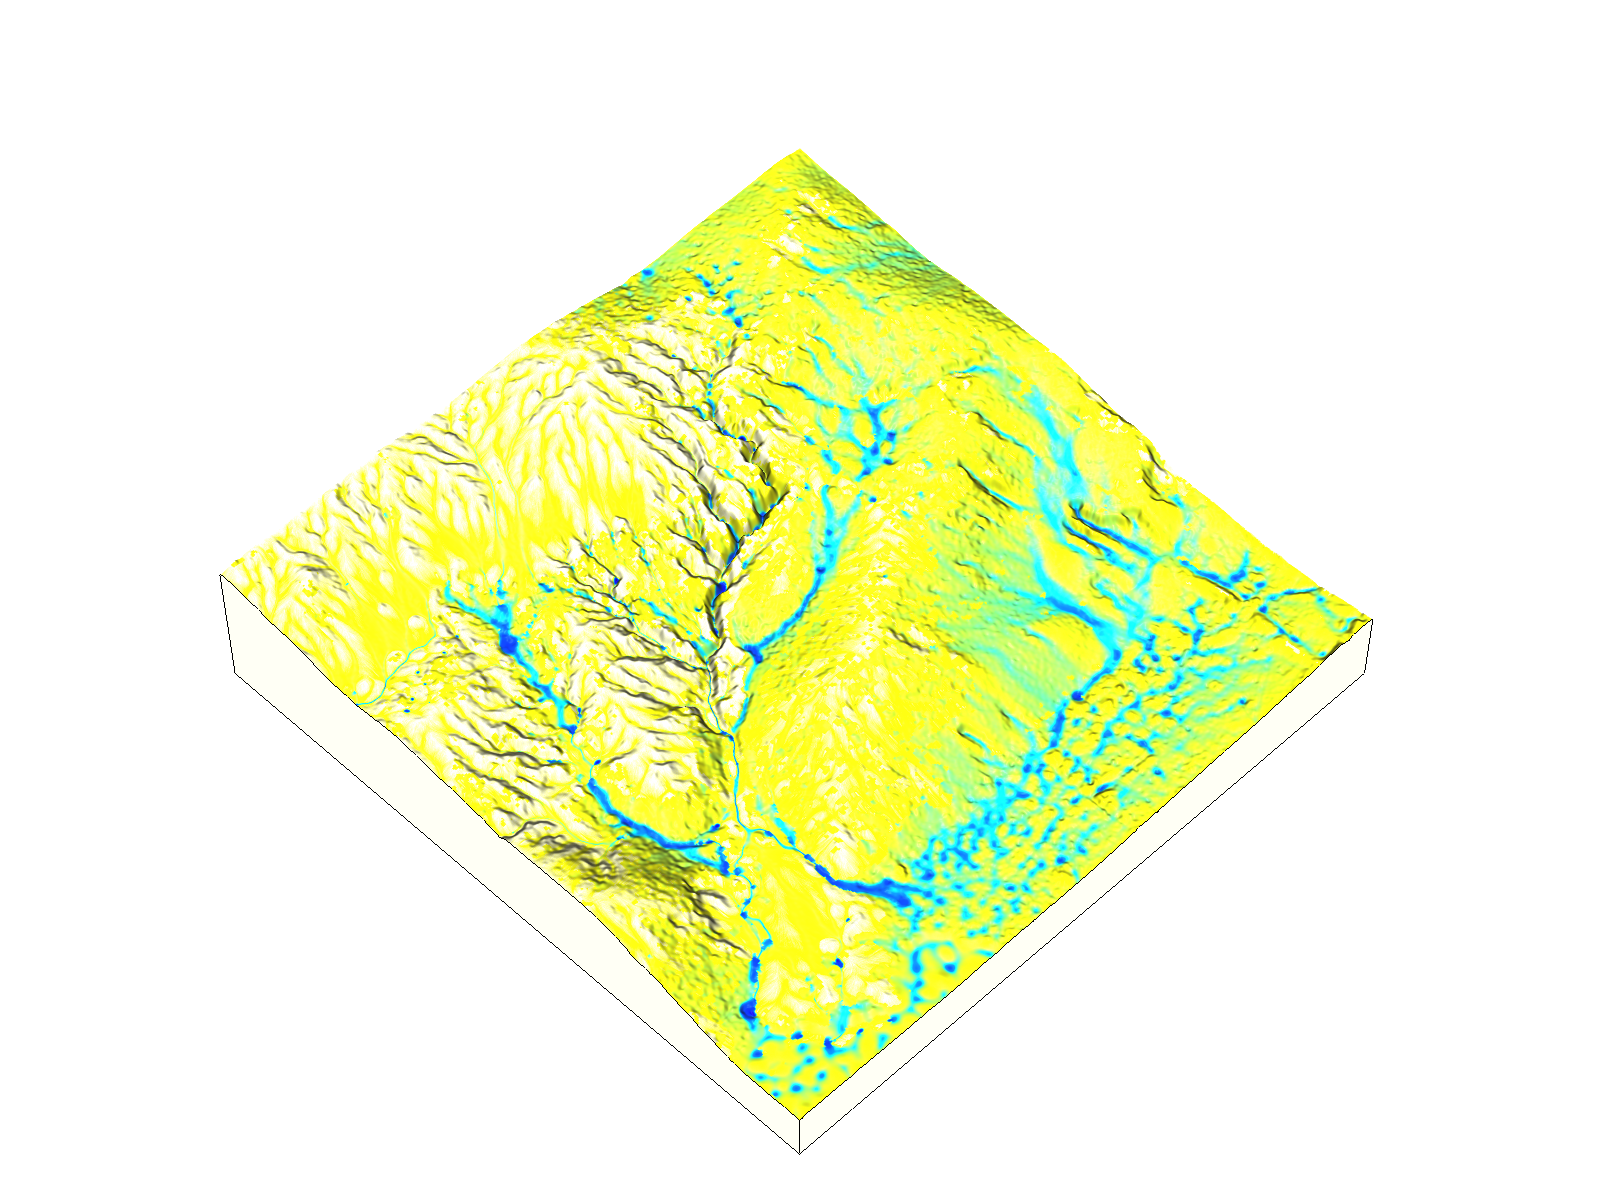
\includegraphics[width=0.5\textwidth]{../images/sample_data_3d/depth_2016.png}
\caption{Shallow overland water flow simulated by SIMWE}
\label{fig:3d}
\end{figure}
%\begin{figure}[t]
%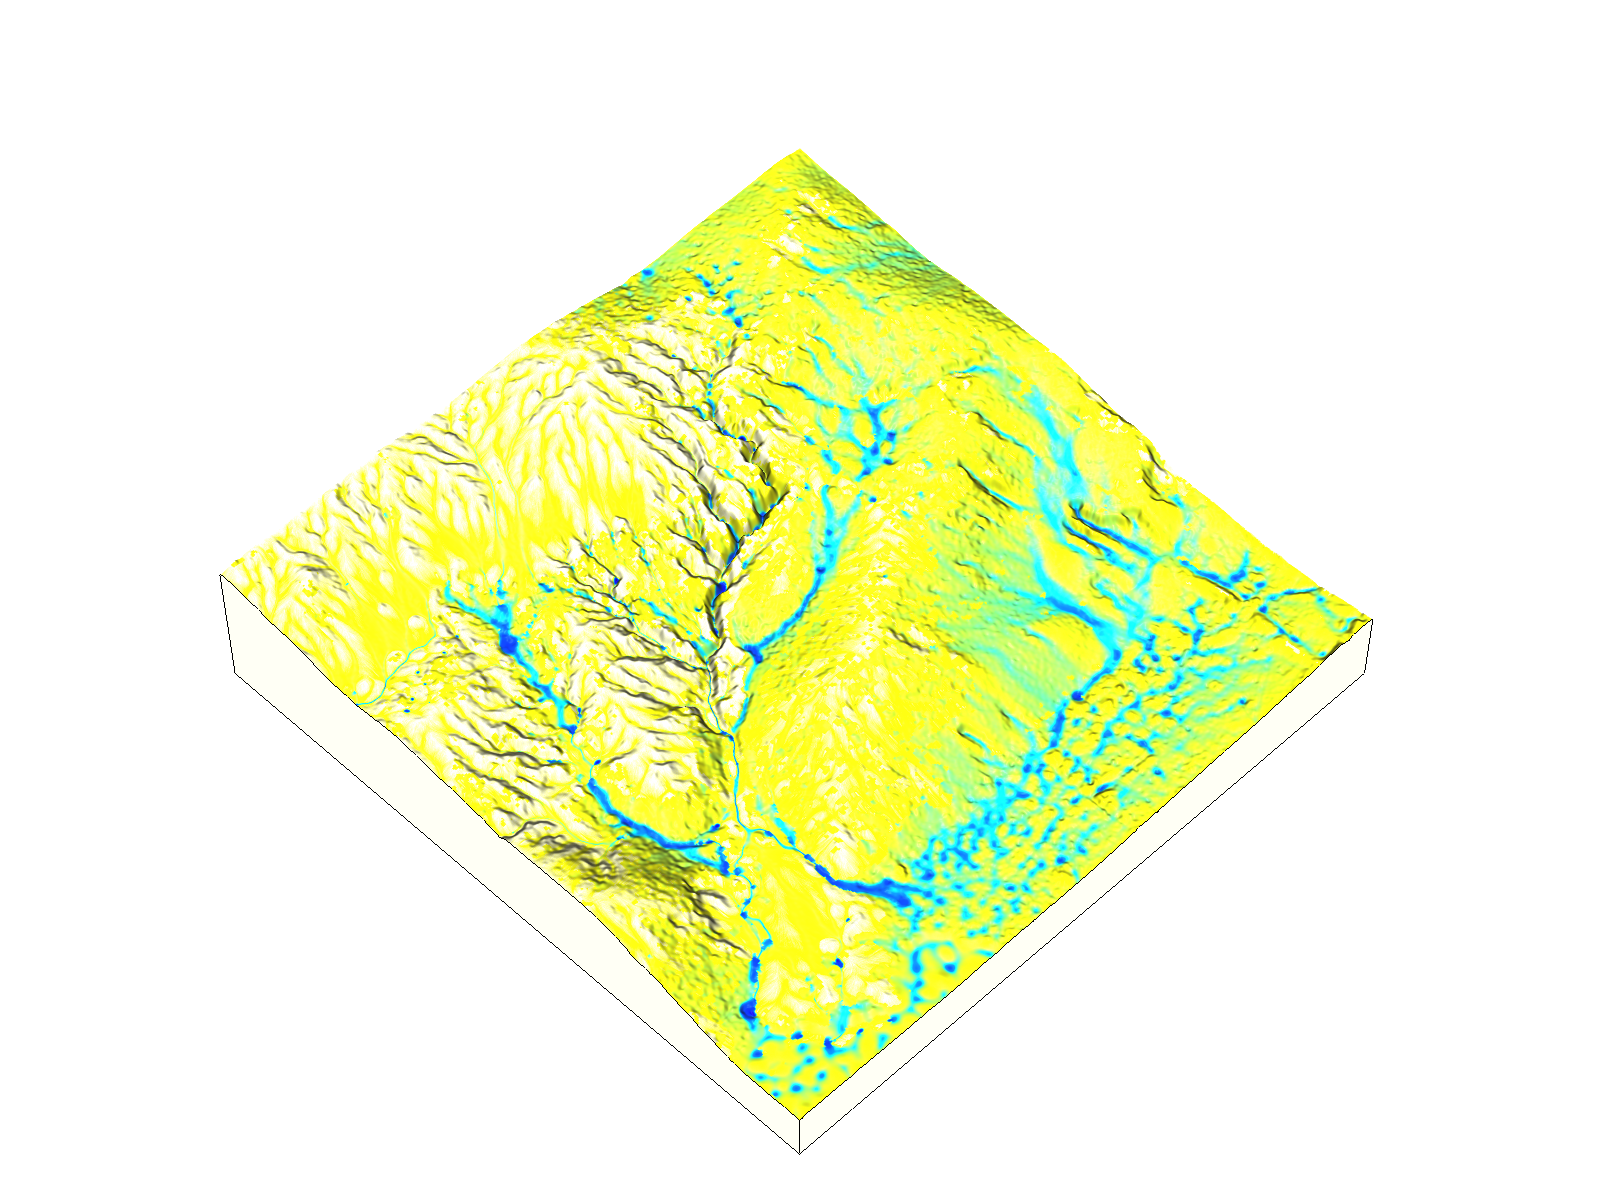
\includegraphics[width=8.3cm]{../images/sample_data_3d/depth_2016.png}
%\caption{Shallow overland water flow simulated by SIMWE}
%\label{fig:3d}
%\end{figure}

% overview
In SIMWE mode 
for each time step
\lowercase{r.sim.terrain}
determines the soil erosion regime,
simulates water and sediment flows, 
and then evolves the topography. 
% erdep
In an erosion-deposition regime 
the model 
computes the partial derivatives of the topography,
simulates shallow water flow and erosion-deposition,
and then evolves the topography based on the erosion-deposition rate
and gravitational diffusion.
% transport limited
The same process is used in
a transport capacity limited regime
except that the topography is evolved based on 
the transport limited erosion-deposition rate
and gravitational diffusion.
% detachment  limited
In a detachment capacity limited regime
the model instead
computes the partial derivatives of the topography,
simulates shallow water flow and sediment flow,
and then evolves the topography based on the sediment flow rate
and gravitational diffusion.
% dynamic versus steady state
The model simulates dynamic landscape evolution 
when the time step is less than the travel time 
for a drop of water or a particle of sediment to cross the landscape.
With longer time steps the model simulates steady state dynamics. 

\subsubsection{Erosion regime}
This model can switch erosion regimes at each time step
based on the rainfall intensity $i_r$
and the balance of the sediment detachment capacity $D_c$
and the sediment transport capacity $T_c$
represented by the first order reaction term $\sigma$ 
which depends on soil and landcover properties.
The detachment capacity is the maximum potential detachment rate by overland flow, while
the sediment transport capacity is the maximum potential sediment flow rate.
%Both are functions of shear stress.

% erosion regime eq.
\begin{equation}
\label{eq:regime}
\sigma = {D_c \over T_c}
\end{equation}
%
{\small
\noindent
where: \\
\noindent
\hspace*{0.5em} $\sigma$  is a first order reaction term ($m^{-1}$)\\
\hspace*{0.5em} $D_c$ is the sediment detachment capacity ($kg~m^{-1}s^{-1}$)\\
\hspace*{0.5em} $T_c$ is the sediment transport capacity ($kg~m^{-1}s^{-1}$)\\
}

%% erosion regime eq.
%\begin{equation}
%\label{eq:regime}
%\sigma({x,y})={D_c({x,y}) \over T_c({x,y})}
%\end{equation}
%
%{\small
%\noindent
%where: \\
%\noindent
%\hspace*{0.5em} $D_c({x,y})$ is the sediment detachment capacity ($kg~m^{-1}s^{-1}$)\\
%\hspace*{0.5em} $T_c({x,y})$ is the sediment transport capacity ($kg~m^{-1}s^{-1}$)\\
%\hspace*{0.5em} $\sigma({x,y})$  is a first order reaction term ($m^{-1}$) \\
%}

When rainfall intensity is very high ($i_r \geq 60 mm~hr^{-1}$)
or $\sigma$ is low ($\sigma \leq 0.01 m^{-1}$),
then the regime is detachment capacity limited. 
%
When rainfall intensity is not very high ($i_r < 60 mm~hr^{-1} $)
and $\sigma$ is high ($\sigma \geq 100 m^{-1}$),
then the regime is transport capacity limited. 
%
When rainfall intensity is not very high ($i_r<60 mm~hr^{-1}$)
and $\sigma$ is neither high nor low ($ 0.01 m^{-1}< \sigma < 100 m^{-1}$),
then there is an erosion-deposition regime. \\

\subsubsection{Shallow water flow}
The SIMWE model
simulates shallow overland water flow 
controlled by spatially variable topographic, soil, landcover, and rainfall parameters
by solving the continuity and momentum equations 
for steady state water flow with a path sampling method. 
Shallow water flow $q(x,y,t)$ can be approximated by
the bivariate form of the St.~Venant equation:

% shallow water flow eq.
\begin{equation}
\label{eq:water}
{\partial h(x,y,t) \over \partial t} =
 i_e(x,y,t) - \nabla ~ q(x,y,t)
\end{equation}
%
{\small
\noindent
where: \\
\noindent
\hspace*{0.5em} $(x,y)$ is the position ($m$)\\
\hspace*{0.5em} $t$ is the time ($s$) \\
\hspace*{0.5em} $h(x,y,t)$ is the depth of overland flow ($m$)\\
\hspace*{0.5em} $i_e(x,y,t)$ is the rainfall excess ($m~s^{-1}$) \\
\hspace*{0.5em} (i.e.~rainfall intensity $-$ infiltration $-$ vegetation intercept)\\
\hspace*{0.5em} $\nabla$ is the divergence of the flow vector field\\
\hspace*{0.5em} $q(x,y,t)$ is the water flow per unit width ($m^2~s^{-1}$). \\
}

Diffusive wave effects can be approximated
so that water can flow through depressions 
by integrating a diffusion term $ \propto \nabla^2 [h^{5/3}(x,y)]$ 
into the solution of the continuity and momentum equations 
for steady state water flow.
This equation is solved using a 
Green's function Monte Carlo path sampling method. 

%  diffuse wave eq.
\begin{equation}
\label{eq:difwater}
-{\varepsilon(x,y)\over 2 }\nabla^2 [h^{5/3}(x,y)]
+\nabla ~ [ h(x,y)~v(x,y)] = i_e(x,y)
\end{equation}
%
{\small
\noindent
 where: \\
 \noindent
 \hspace*{0.5em} $\varepsilon(x,y)$ is a spatially variable diffusion coefficient. \\
}

\subsubsection{Sediment flow}
In SIMWE the sediment flow rate $q_s(x,y,t)$ is estimated 
as a function of water flow and sediment concentration:

%sediment flow equation
\begin{equation}\label{eq:sedflow} 
q_s(x,y,t) = \rho_s(x,y,t) ~ q(x,y,t)
\end{equation}
%
{\small
\noindent
where: \\
\hspace*{0.5em} $q_s(x,y,t)$ is the sediment flow rate per unit width ($kg~m^{-1}s^{-1}$)\\
\hspace*{0.5em} $\rho_s(x,y,t)$ is sediment mass density ($kg~m^{-3}$).\\
%\hspace*{0.5em} $q(x,y,t)$ is unit flow discharge vector ($m^{2} s^{-1}$) \\
%\hspace*{0.5em} (i.e.~ the direction and rate of water flow per unit width)\\
}

\subsubsection{Erosion-deposition}
In SIMWE 
the net erosion-deposition rate is estimated
using the bivariate form of sediment continuity equation
to model sediment storage and flow 
based on effective sources and sinks.
Net erosion-deposition $d_s(x,y,t)$
-- the difference between sources and sinks --
is approximated by
the steady state sediment flow equation with diffusion:

% erosion-deposition equation
\begin{equation}\label{eq:sediment} 
d_s(x,y,t) = 
{\partial [\rho_sc(x,y,t)h(x,y,t)] \over \partial t} +
\nabla ~ q_s(x,y,t)
\end{equation}
%
{\small
\noindent
where: \\
\hspace*{0.5em} $d_s(x,y,t)$ is net erosion-deposition $(kg ~ m^{-2} s^{-1})$.\\
%\hspace*{0.5em} $q_s(x,y,t)$ is the sediment flow rate per unit width ($kg~m^{-1}s^{-1}$)\\
%\hspace*{0.5em} $\rho_s(x,y,t)$ is sediment mass density ($kg~m^{-3}$).\\
}

%\begin{equation}\label{eq:sediment} 
%D(x,y,t) = \mathrm{source - sinks} =
%{\partial [\rho_sc(x,y,t)h(x,y,t)] \over \partial t} +
%\nabla ~ q_s(x,y,t)
%\end{equation}

%Sources and sinks of sediment are assumed to be proportional to
%the difference between sediment transport capacity
%and the sediment flow rate: 
%\begin{equation}\label{eq:sources_sinks} 
%d_s = \sigma [T_c  - |q_s|]
%\end{equation}

% ADD transport limited erosion-deposition

\subsubsection{Landscape evolution}
The simulated change in elevation $\Delta z(x,y,t)$ due to water erosion and deposition
is a function of
the change in time, the net erosion-deposition rate, and the sediment mass density 
\cite{Mitasova2013}:

% landscape evolution equation
% change in elevation (m) = change in time (s) * net erosion-deposition (kg/m^2s) / sediment mass density (kg/m^3)
\begin{equation}
\label{eq:evolution} 
{\Delta z(x,y,t) = \Delta t ~ d_s(x,y,t) ~ \rho_s^{-1} }
\end{equation}

%{\small
%\noindent
%where: \\
%\noindent
%\hspace*{0.5em} $\Delta z =$ change in elevation $(m)$ \\
%\hspace*{0.5em} $d_s =$ net erosion-deposition $(kg ~ m^{-2} s^{-1})$ \\
%\hspace*{0.5em} $\rho_s c(x,y,t)$ = sediment mass density $(kg ~m^{-3})$\\ %[kg/m$^3$]
%\hspace*{0.5em} $\rho_s =$ sediment mass density $(kg ~m^{-3})$ \\
%}

% detachment limited landscape evolution
In a detachment limited erosion regime
the simulated change in elevation $\Delta z(x,y,t)$
is a function of
the change in time, the sediment flow rate, and the mass of water carried sediment per unit area
\cite{Mitasova2013}:

% change in elevation (m) = change in time (s) * sediment flux (kg/ms) / mass of sediment per unit area (kg/m^2)
\begin{equation}
\label{eq:flux_evolution} 
{\Delta z(x,y,t) = \Delta t ~ q_s(x,y,t) ~ \varrho_s^{-1} } 
\end{equation}
% \varrho_s(r)^{-1}
%
{\small
\noindent
where: \\
\noindent
%\hspace*{0.5em} $\Delta z =$ change in elevation $(m)$ \\
%\hspace*{0.5em} $q_s =$ sediment flux $(kg ~ m^{-1} s^{-1})$ \\
\hspace*{0.5em} $\varrho_s$ is the mass of sediment per unit area $(kg ~ m^{-2})$.\\
}

% gravitational diffusion
\noindent
Gravitational diffusion is then applied to the evolved topography
to simulate the settling of sediment particles. 
The simulated change in elevation $\Delta z(x,y,t) $ due to gravitational diffusion 
is a function of the change in time, the sediment mass density, 
the gravitational diffusion coefficient, and topographic divergence 
-- i.e.~the sum of the second order derivatives of elevation
\cite{thaxton2004}:

%gravitional diffusion eq.
% change in elevation (m) = elevation (m) - (change in time (s) / sediment mass density (kg/m^3) * gravitational diffusion coefficient (m^2/s) * divergence (m^-1))
\begin{equation}
\label{eq:grav_diffusion} 
{\Delta z(x,y,t) = \Delta t ~ \rho_s^{-1} ~ \varepsilon_g ~ \nabla(x,y,t)}
\end{equation}
%
{\small
\noindent
where: \\
\noindent
%\hspace*{0.5em} $\Delta z =$ change in elevation $(m)$ \\
%\hspace*{0.5em} $\rho_s c(x,y,t)$ = sediment mass density $(kg ~m^{-3})$\\ %[kg/m$^3$]
%\hspace*{0.5em} $\rho_s =$ sediment mass density $(kg ~m^{-3})$ \\
\hspace*{0.5em} $\varepsilon_g$ is the gravitational diffusion coefficient $(m^{2} s^{-1})$\\ %$(m^{-2} s^{-1})$
\hspace*{0.5em} $\nabla(x,y,t)$ is the topographic divergence $(m^{-1})$.\\
}


\conclusions  %% \conclusions[modified heading if necessary]
...

%% The following commands are for the statements about the availability of data sets and/or software code corresponding to the manuscript.
%% It is strongly recommended to make use of these sections in case data sets and/or software code have been part of your research the article is based on.

\codeavailability{TEXT} %% use this section when having only software code available


\dataavailability{TEXT} %% use this section when having only data sets available


\codedataavailability{TEXT} %% use this section when having data sets and software code available


\sampleavailability{TEXT} %% use this section when having geoscientific samples available



\appendix
\section{}    %% Appendix A

\subsection{}     %% Appendix A1, A2, etc.


\noappendix       %% use this to mark the end of the appendix section

%% Regarding figures and tables in appendices, the following two options are possible depending on your general handling of figures and tables in the manuscript environment:

%% Option 1: If you sorted all figures and tables into the sections of the text, please also sort the appendix figures and appendix tables into the respective appendix sections.
%% They will be correctly named automatically.

%% Option 2: If you put all figures after the reference list, please insert appendix tables and figures after the normal tables and figures.
%% To rename them correctly to A1, A2, etc., please add the following commands in front of them:

\appendixfigures  %% needs to be added in front of appendix figures

\appendixtables   %% needs to be added in front of appendix tables

%% Please add \clearpage between each table and/or figure. Further guidelines on figures and tables can be found below.



\authorcontribution{TEXT} %% it is strongly recommended to make use of this section

\competinginterests{TEXT} %% this section is mandatory even if you declare that no competing interests are present

\disclaimer{TEXT} %% optional section

\begin{acknowledgements}
TEXT
\end{acknowledgements}


% REFERENCES
\bibliographystyle{copernicus}
\bibliography{landscape_evolution.bib}


%% The reference list is compiled as follows:

%\begin{thebibliography}{}
%
%\bibitem[AUTHOR(YEAR)]{LABEL1}
%REFERENCE 1
%
%\bibitem[AUTHOR(YEAR)]{LABEL2}
%REFERENCE 2
%
%\end{thebibliography}

%% Since the Copernicus LaTeX package includes the BibTeX style file copernicus.bst,
%% authors experienced with BibTeX only have to include the following two lines:
%%
%% \bibliographystyle{copernicus}
%% \bibliography{example.bib}
%%
%% URLs and DOIs can be entered in your BibTeX file as:
%%
%% URL = {http://www.xyz.org/~jones/idx_g.htm}
%% DOI = {10.5194/xyz}


%% LITERATURE CITATIONS
%%
%% command                        & example result
%% \citet{jones90}|               & Jones et al. (1990)
%% \citep{jones90}|               & (Jones et al., 1990)
%% \citep{jones90,jones93}|       & (Jones et al., 1990, 1993)
%% \citep[p.~32]{jones90}|        & (Jones et al., 1990, p.~32)
%% \citep[e.g.,][]{jones90}|      & (e.g., Jones et al., 1990)
%% \citep[e.g.,][p.~32]{jones90}| & (e.g., Jones et al., 1990, p.~32)
%% \citeauthor{jones90}|          & Jones et al.
%% \citeyear{jones90}|            & 1990



%% FIGURES

%% When figures and tables are placed at the end of the MS (article in one-column style), please add \clearpage
%% between bibliography and first table and/or figure as well as between each table and/or figure.


%% ONE-COLUMN FIGURES

%%f
%\begin{figure}[t]
%\includegraphics[width=8.3cm]{FILE NAME}
%\caption{TEXT}
%\end{figure}
%
%%% TWO-COLUMN FIGURES
%
%%f
%\begin{figure*}[t]
%\includegraphics[width=12cm]{FILE NAME}
%\caption{TEXT}
%\end{figure*}
%
%
%%% TABLES
%%%
%%% The different columns must be seperated with a & command and should
%%% end with \\ to identify the column brake.
%
%%% ONE-COLUMN TABLE
%
%%t
%\begin{table}[t]
%\caption{TEXT}
%\begin{tabular}{column = lcr}
%\tophline
%
%\middlehline
%
%\bottomhline
%\end{tabular}
%\belowtable{} % Table Footnotes
%\end{table}
%
%%% TWO-COLUMN TABLE
%
%%t
%\begin{table*}[t]
%\caption{TEXT}
%\begin{tabular}{column = lcr}
%\tophline
%
%\middlehline
%
%\bottomhline
%\end{tabular}
%\belowtable{} % Table Footnotes
%\end{table*}
%
%%% LANDSCAPE TABLE
%
%%t
%\begin{sidewaystable*}[t]
%\caption{TEXT}
%\begin{tabular}{column = lcr}
%\tophline
%
%\middlehline
%
%\bottomhline
%\end{tabular}
%\belowtable{} % Table Footnotes
%\end{sidewaystable*}

%%% MATHEMATICAL EXPRESSIONS
%
%%% All papers typeset by Copernicus Publications follow the math typesetting regulations
%%% given by the IUPAC Green Book (IUPAC: Quantities, Units and Symbols in Physical Chemistry,
%%% 2nd Edn., Blackwell Science, available at: http://old.iupac.org/publications/books/gbook/green_book_2ed.pdf, 1993).
%%%
%%% Physical quantities/variables are typeset in italic font (t for time, T for Temperature)
%%% Indices which are not defined are typeset in italic font (x, y, z, a, b, c)
%%% Items/objects which are defined are typeset in roman font (Car A, Car B)
%%% Descriptions/specifications which are defined by itself are typeset in roman font (abs, rel, ref, tot, net, ice)
%%% Abbreviations from 2 letters are typeset in roman font (RH, LAI)
%%% Vectors are identified in bold italic font using \vec{x}
%%% Matrices are identified in bold roman font
%%% Multiplication signs are typeset using the LaTeX commands \times (for vector products, grids, and exponential notations) or \cdot
%%% The character * should not be applied as mutliplication sign

%%% EQUATIONS
%
%%% Single-row equation
%
%\begin{equation}
%
%\end{equation}

%%% Multiline equation
%
%\begin{align}
%& 3 + 5 = 8\\
%& 3 + 5 = 8\\
%& 3 + 5 = 8
%\end{align}

%%% ALGORITHM
%
%\begin{algorithm}
%\caption{...}
%\label{a1}
%\begin{algorithmic}
%...
%\end{algorithmic}
%\end{algorithm}

%%% PHYSICAL UNITS
%%%
%%% Please use \unit{} and apply the exponential notation


\end{document}
